\documentclass[twocolumn]{revtex4-1}
\usepackage{amssymb}
\usepackage{amsmath}
\usepackage{graphicx}
\usepackage[pdfpagelabels,pdftex,bookmarks,breaklinks]{hyperref}
\usepackage{tikz}
\usepackage[all]{hypcap}
\hypersetup{colorlinks,citecolor=blue,urlcolor=blue,linkcolor=blue}

\def\sectionautorefname{Section}

\begin{document}
\title{Halving the cost of quantum addition}
\author{Craig Gidney}
\affiliation{Google, Santa Barbara, CA 93117, USA}
\email{craiggidney@google.com}

\begin{abstract}
We improve the number of T gates needed to perform an $n$-bit adder from $8n + O(1)$ \citep{Amy2013, Cuccaro2004, AustinDiscussionsAndEmails2017} to $4n + O(1)$.
We do so via a ``temporary logical-AND" construction, which uses four T gates to store the logical-AND of two qubits into an ancilla and zero T gates to later erase the ancilla.
Temporary logical-ANDs are a generally useful tool when optimizing T-counts.
They can be applied to integer arithmetic, modular arithmetic, rotation synthesis, the quantum Fourier transform, Shor's algorithm, Grover oracles, and many other circuits.
Because T gates dominate the cost of quantum computation based on the surface code, and temporary logical-ANDs are widely applicable, our constructions represent a significant reduction in projected costs of quantum computation.
We also present an $n$-bit controlled adder circuit with T-count of $8n + O(1)$, a temporary adder that can be computed for the same cost as the normal adder but whose result can be kept until it is later uncomputed without using T gates, and discuss some other constructions whose T-count is improved by the temporary logical-AND.
\end{abstract}

\maketitle

\section*{Introduction}

The surface code \citep{Brav98,Denn02,Raus07,Raus07d,Fowler2012} is a quantum error correcting code that works on a 2D nearest-neighbour array of qubits and achieves a threshold error rate of approximately 1\%.
This makes the surface code a likely component in the architecture of future error corrected quantum computers, because 2D arrays of qubits with nearest-neighbor connections are possible with many qubit technologies \citep{Schl11,Bare13,Gamb17,Leik17,Laht17} and other well understood error correcting codes either have lower thresholds or require stronger connectivity.

One of the downsides of the surface code is that it has no cheap mechanism to apply non-Clifford operations such as $T$ gates.
Instead, $T$ gates are performed by distilling and consuming $|A\rangle = \frac{1}{\sqrt{2}} (|0\rangle + e^{i \pi/4} |1\rangle)$ states.
Consuming an $|A\rangle$ state to perform a T gate is simple, but distilling $|A\rangle$ states has significant cost.
Because T gates are so expensive for the surface code, and the surface code is a likely component of future quantum computers, it is important to consider and optimize the number of T gates used by quantum circuits.
Optimizing the T-count of basic elements of quantum circuits, such as the construction of adders and Toffoli gates, is particularly important because any improvement is widely applicable.

The textbook construction of a Toffoli gate uses seven T gates \citep{Nielsen2009}.
When Toffoli operations are paired, i.e. when an initial Toffoli operation is later uncomputed by a second Toffoli operation, each Toffoli in the pair can omit three of the T gates from the textbook construction.
This introduces phase errors but, assuming intermediate operations aren't sensitive to the phase errors, the second Toffoli gate can uncompute the phase errors while uncomputing the state permutation \citep{Barenco1995, Nielsen2009}.
It is also possible to reduce the T-count of an unpaired Toffoli gate to 4 by using an ancilla qubit and a classically conditioned fixup operation \citep{Jones2013}.

The Cuccaro adder uses $2n + O(1)$ Toffoli gates \citep{Cuccaro2004}.
Existing constructions implement the Cuccaro adder's Toffolis using $8n + O(1)$ T gates \citep{Barenco1995, Cuccaro2004, Amy2013}.
This T-count can be achieved either by applying the ancilla-and-fixup construction from \citep{Jones2013} to each individual Toffoli gate, or by noting that all but one of the adder's Toffoli gates appear in compute/uncompute pairs and then applying the matched-phase-error construction from \citep{Barenco1995, Nielsen2009} to each pair.

The leading factor of 8 in the T-count of an $n$-bit adder has stood for over a decade \citep{Barenco1995, Cuccaro2004, AustinDiscussionsAndEmails2017}.
We improve the leading factor with a construction based on the temporary logical-AND, which combines ideas from both the matched-phase-error construction and the ancilla-and-fix-up construction.
The temporary logical-AND halves the number of T gates needed to perform Toffoli gates that appear in compute/uncompute pairs, and thereby halves the T-count of the Cuccaro adder from $8n + O(1)$ to $4n + O(1)$.

\begin{figure}
  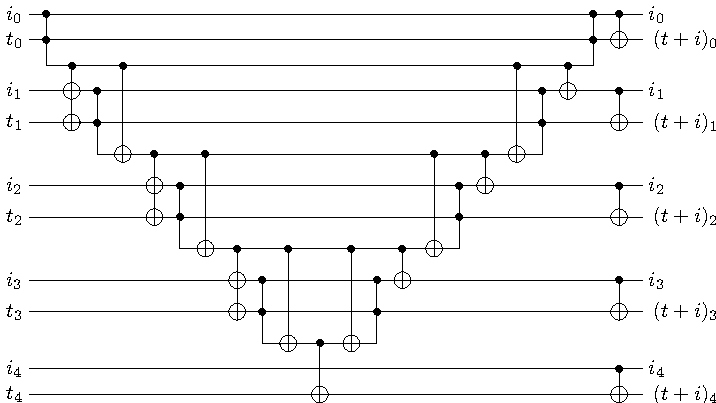
\includegraphics[width=\linewidth]{figures/adder.pdf}
  \caption{
	A 5-bit adder with T-count of 16.
	Uses Clifford operations, four logical-AND computations each with a T-count of 4, and four logical-AND erasures requiring no T gates.
	Generalizes to an $n$-bit adder with a T-count of $4n - 4$.
	See \autoref{fig:adder-building-block} for the adder building-block and \autoref{fig:temporary-logical-AND} for the logical-AND computation and uncomputation circuits.
  }
  \label{fig:adder}
\end{figure}


\section*{Results}

In \autoref{fig:adder}, we present a 5-bit adder with a T-count of 16.
It performs 4 temporary logical-ANDs, each with a T-count of 4.
All other operations are Clifford operations, with no T-count.

The building block of our adder is shown in \autoref{fig:adder-building-block}.
We construct $n$-bit adders by nesting $n$ copies of the building block inside of each other.
The outer-most and inner-most blocks (which act on the low bit and high bit respectively) are then specialized based on the fact that they either have no carry input or no carry output.

\begin{figure}
  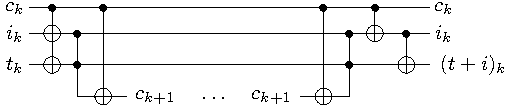
\includegraphics[width=\linewidth]{figures/adder-building-block.pdf}
  \caption{
	Our adder circuit building-block, with a T-count of 4.
	A variant of the Cuccaro adder building-block \citep{Cuccaro2004}.
  }
  \label{fig:adder-building-block}
\end{figure}

Our adder uses temporary logical-AND operations, which we draw as wires emerging out of a pair of controls then later merging into the same pair of controls.
\autoref{fig:temporary-logical-AND} shows how we compute the logical-AND of the two controls (which we draw as a wire emerging from two controls then heading rightward), and also the corresponding uncomputation (which we draw as a wire turning upward into two controls).

Computing the temporary logical-AND has a T-count of 4, but uncomputing it has a T-count of 0.
This asymmetry is due to the fact that measurement is not reversible.
The uncomputation uses measurement in a way that the computation cannot.


\autoref{fig:other-adder-building-blocks} shows the building-blocks for two variations on our adder: a controlled adder and a temporary adder.

Some additions, such as the ones performed by the multiplications within the modular exponentiation in Shor's algorithm, are conditioned on a control qubit.
Our controlled adder reduces the cost of these additions from $21n + O(1)$ \citep{Coreas2017} to $8n + O(1)$.

Temporary adders are useful when a circuit is going to compute an addition, then later uncompute it.
Instead of paying $4n + O(1)$ T gates to compute an addition, and then $4n + O(1)$ more T gates to uncompute the addition with a subtraction, our temporary adder stops halfway through the normal addition (after all the logical-ANDs have been computed, but before they've been uncomputed) and applies a few cleanup operations so that the sum is available for use.
When the sum is no longer needed, the partially-performed addition is uncomputed instead of completed.

\begin{figure}
  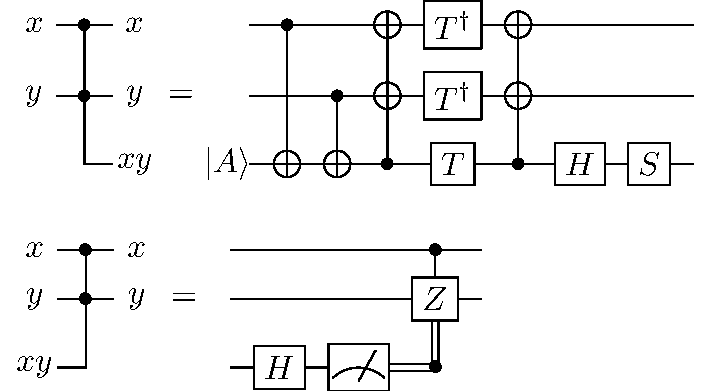
\includegraphics[width=\linewidth]{figures/temporary-logical-and.pdf}
  \caption{
	How to compute and uncompute the logical-AND of two qubits.
	The computation circuit (top) has a T-count of 4 and a T-depth of 1.
	Note that the $|A\rangle$ state input contributes to the T-count, because $|A\rangle$ states are the resource used to perform T gates.
	The uncomputation circuit (bottom) uses a measure-and-fixup approach \cite{Jones2013} that requires only Clifford gates, and so has a T-count of zero.
    \\
    An alternative uncomputation construction is to simply do the reverse of the computation circuit.
    This alternative approach has a net T-count of 2 (because an $|A\rangle$ state is recovered).
    The resulting temporary logical-AND with a T-count of 6 would still be an improvement on existing work, but would be inferior to the measure-and-fixup approach shown above.
  }
  \label{fig:temporary-logical-AND}
\end{figure}

Decreasing the T-count of addition reduces the T-count of any construction based on addition.
For example, in \citep{Fowler2012} it is estimated that factoring a 2048-bit number on a surface-code-based quantum computer would take 27 hours and $2 \cdot 10^{12}$ distilled $|A\rangle$ states.
The time estimate is based on Toffolis having a T-depth of 3, and the $|A\rangle$ count estimate is based on Toffolis having a T-count of 7.
Because Shor's algorithm is dominated by the cost of controlled additions, our techniques (and previous work) reduce the average T-count and T-depth of its Toffolis to $\sim 2.7$ and $1$ respectively.
This reduces the time estimate to 9 hours and the count estimate to $8 \cdot 10^{11}$ distilled $|A\rangle$ states.

On top of reducing the T-count of obviously-related classical operations like multiplication and exponentiation, reducing the T-count of addition also reduces the T-count of quantum-specific operations such as rotating qubits.

For example, our improved adder allows the operation $R_Z(\theta)$ to be applied to $n$ qubits with a T-cost of $4n + O(\text{poly}(\lg \frac{1}{\epsilon}) \lg n)$ as follows.
First, iteratively apply our temporary adder to combine the target qubits into a single binary register storing their Hamming weight.
This takes $4n + O(\lg n)$ T gates to do.
Then, for each position $p$ in the Hamming weight register, synthesize and apply the operation $R_Z(\theta \cdot 2^p)$ to the register qubit at that position.
This uses a number of T gates proportional to some polynomial of the desired bit precision, times the number of bits in the Hamming weight register.
The Hamming weight register is exponentially smaller than $n$, so this cost is negligible for large $n$.
Finally, uncompute the Hamming weight register (using no T gates).
This applies the $n$ desired $R_Z(\theta)$ operations.

Another quantum operation that can be implemented via an adder is the $n$-qubit phase gradient operation $\text{Grad}_n = \sum_{k=0}^{2^n-1} e^{2 i \pi k / 2^n} |k\rangle \langle k|$.
Normally this operation would be implemented by separately applying the operation $R_Z(\pi 2^{-p})$ to each qubit of the target register, where $p$ is the qubit's index in the register and the number of T gates needed for each rotation depends on the maximum per-gate error $\epsilon$.
However, assuming a ``phase gradient register" prepared in the state $2^{-b/2} \sum_{k=0}^{2^b-1} e^{-2 i \pi k / 2^b} |k\rangle$ is available, the phase gradient operation can be performed via addition.
Add the target register into the phase gradient register, and phase kickback will apply the $\text{Grad}_n$ operation to the target.
This construction performs phase gradients using $4n + O(1)$ T gates.
This T-count is interesting because it appears to be independent of $\epsilon$ despite the phase gradient operation involving arbitrarily small rotations.
However, there are three ways in which our phase gradient construction's cost does depend on $\epsilon$.
First, $\epsilon$ still bounds the minimum quality of the $|A\rangle$ states powering the T gates.
Second, large phase gradients can be truncated down to a size $n_{\text{max}}$ asymptotically equal to $\lg \lg \frac{1}{\epsilon}$.
Third, initializing the reusable phase gradient register has a one-time cost of $O(n_{\text{max}} \cdot \text{poly}(\lg \frac{1}{\epsilon}))$ T gates.


\begin{figure}
  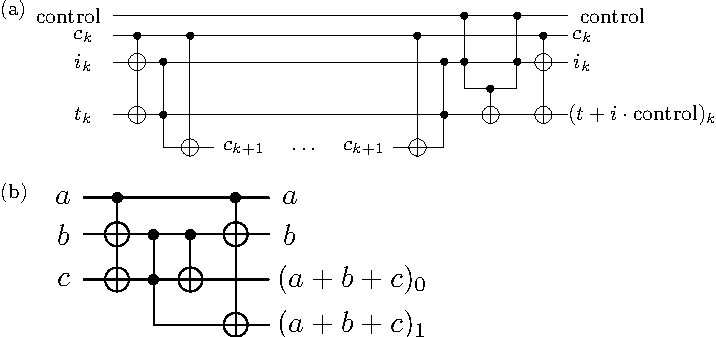
\includegraphics[width=\linewidth]{figures/other-adder-building-blocks.pdf}
  \caption{
	Variations on our adder construction.
	(a) is a controlled-adder building-block with a T-count of 8.
	The addition will only occur when the control is on.
	(b) is a temporary-adder building-block with a T-count of 4.
	Has the same T-count as a normal addition, but makes the result available before any uncomputation steps are needed.
  }
  \label{fig:other-adder-building-blocks}
\end{figure}

The temporary logical-AND is useful for optimizing an even wider variety of circuits than addition is.
Whenever Toffoli gates appear in compute/uncompute pairs, and intermediate operations are not sensitive to phase errors on the controls of the Toffoli gate (i.e. the condition in \autoref{fig:paired-toffoli-replacement-rule} is satisfied), it is possible to save 4 T gates by replacing the pair of Toffoli gates with a temporary logical-AND.

\begin{figure}
  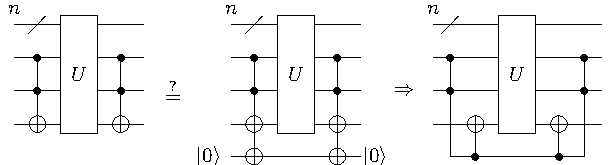
\includegraphics[width=\linewidth]{figures/paired-toffoli-replacement-rule.pdf}
  \caption{
	A sufficient condition for replacing a pair of Toffoli gates with a temporary logical-AND, saving 4 T gates.\\
	1) The later Toffoli gate must be uncomputing the earlier Toffoli gate.\\
	2) Intermediate operations must not be sensitive to the presence of the entangled ancilla.
  }
  \label{fig:paired-toffoli-replacement-rule}
\end{figure}

For example, a simple way to construct Grover oracles starts by translating a classical predicate into a classical reversible circuit made with Toffoli gates.
This reversible circuit is then used on a quantum computer to compute an output qubit, and a Z gate is applied to the output qubit before the circuit is run in reverse to uncompute the output qubit.
Every Toffoli gate generated by this construction is part of a compute/uncompute pair (each Toffoli in the computation will match a Toffoli in the uncomputation).
Using temporary logical-ANDs, instead of individually translating each Toffoli gate into T gates, halves the T-count of this approach to constructing Grover oracles.

As another example, note that the temporary logical-AND can perform NOT gates with many controls by iteratively combining the controls down to a single representative ancilla.
The representative ancilla is then used to control a CNOT onto the target qubit.
Overall this takes $4n-4$ T gates, equivalent to previous work \cite{Jones2013}.
As when replacing Toffoli gates in compute/uncompute pairs with a temporary logical-AND, the ancilla representing the $n$ controls should be kept and used multiple times whenever possible (instead of being uncomputed and recomputed).

Finally, we note that Toffolis also appear in compute/uncompute pairs in quantum circuits rooted in physics instead of abstract mathematics.
For example, we used temporary logical-ANDs to cut the projected T-count of a step in a simulation algorithm under development by nearly 30\% \citep{RyanEmails2017}.


\section*{Discussion}

For over a decade, the T-count of addition has been $8n + O(1)$ \citep{Amy2013, Barenco1995, Cuccaro2004}.
In this paper we showed how to halve the leading factor of this cost by replacing Toffolis in compute/uncompute pairs with temporary logical-ANDs.
The temporary logical-AND is a basic circuit construction widget that can be used in many circuits, and a good example of measurement breaking the symmetry between computation and uncomputation (allowing one to be more efficient than the other).
We demonstrated how to optimize the T-count of a few tasks using our adder and the temporary logical-AND, but there are many other low hanging applications.

It is interesting to consider if addition or temporary logical-ANDs can be done with still fewer T gates.
\autoref{fig:synthesize-t-gates-from-temporary-logical-and} presents a simple proof that the T-count of the temporary logical-AND is at least 2.
Although we suspect the true lower bound is 4, we also expect that there are special cases with lower T-counts.
For example, if a task involves repeating an action several times (e.g. counting by repeatedly conditionally incrementing a register), T gates from Toffolis in uncomputation work at the end of one repetition may cancel against T gates from Toffolis in computation work at the start of the next repetition.

\begin{figure}
  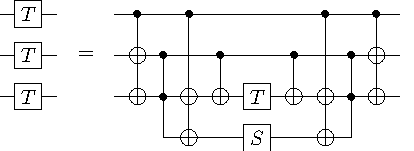
\includegraphics[width=\linewidth]{figures/synthesize-t-gates-from-temporary-logical-and.pdf}
  \caption{
	Three T gates can be synthesized by performing a temporary logical-AND, one T gate, and various Clifford operations.
	Clifford operations can't produce T gates, so the extra T gates must be coming from the temporary logical-AND.
	This proves that performing the temporary logical-AND requires at least two T gates.
  }
  \label{fig:synthesize-t-gates-from-temporary-logical-and}
\end{figure}

Regardless of whether there will be further T-count improvements for operations as basic as Toffoli gates appearing in pairs, it is clear that many other kinds of T-count optimizations are waiting to be found.
Not just in the construction of basic low-level operations, but in medium-level constructions, high-level constructions, lower-than-circuit level constructions, and generally across the whole technology stack that will be needed to perform error corrected quantum computation with the surface code for the first time.


\section*{Acknowledgements}

We thank Austin Fowler for sampling the opinions of other researchers, for assistance locating references, and for comments that significantly improved this paper.
We thank Dave Bacon and Dmitri Maslov for comments that significantly improved this paper.


\bibliographystyle{plainnat}
\bibliography{citations}

\end{document}
